\section{Ejemplo: el estimador de Nadaraya-Watson}
Presentamos a continuación un ejemplo del mecanismo de atención aplicada a problemas de regresión: el estimador de Nadaraya-Watson \cite{watson1964smooth, nadaraya1964estimating}.

Nos encontramos en el marco habitual de un problema de regresión: disponemos de un conjunto de características observadas \( \{ x_{i} : i = 1, \dots, m \} \) con \( x_{i}  \in \real{n} \} \) y de un vector \( y = (y_1, \dots, y_m) \) que recoge el valor de la variable objetivo para cada una de las observaciones. Dada una nueva observación \( x_{0} \), queremos aproximar el valor de la variable objetivo \( y_{0} \) mediante un estimador \( \widehat{y}_{0} \).

Definimos la base de datos \( \mathcal{D} = \left\{ (x_{i}, y_{i}) : i = 1, \dots, m \right\} \). Consideramos una función \( \alpha \) normalizada entre \( 0 \) y \( 1 \), esto es:
\[
    \alpha(q, k_{i}) = \frac{a(q, k_{i})}{\sum_j \alpha(q, k_{j}) }
\]
para alguna función \( a : \real{n} \times \real{n} \to \realo \). La atención de \( q \) sobre \( \mathcal{D} \) es:
\[
    \attention(q, \mathcal{D}; \alpha) = \sum_i  \alpha(q, k_{i}) v_{i} = \sum_i \frac{a(q, k_{i})}{\sum_j \alpha(q, k_{j})} v_{i}
\]

Podemos ahora aproximar \( y_{0} \) mediante el estimador 
\begin{equation}\label{eq:kde}
    \widehat{y}_{0} = \left\langle y, \attention(x_{0}, \mathcal{D}; \alpha) \right\rangle
\end{equation}

La \cref{fig:regression} muestra el resultado de estimar la distribución de \( n = 100 \) puntos de la forma \( (x_{i}, y_{i}) \) siendo \( (x_{i}) \) una sucesión ordenada de puntos en \( [0, 5] \), \( y_{i} = x_{i} + \sin(x_{i}) + \epsilon \) con \( \epsilon \sim \mathcal{N}(0, 1) \). Para ello, utilizamos una partición equiespaciada \( x^\text{val}_{i} \) de \( [0, 5] \) con 100 puntos y estimamos \( \widehat{y}^\text{val} \) usando la \cref{eq:kde} con varios \textit{kernel} de similitud distintos:
\[
    \begin{split}\begin{aligned}
    a(q, k) & = \exp\left(-\frac{1}{2} \|q - k\|^2 \right) && \mathrm{Gaussiana} \\
    a(q, k) & = \begin{cases}
        1 &\text{ si } \|q - k\| \leq 1 \\
        0 &\text{ si no}
    \end{cases} && \mathrm{Boxcar}
    \\
    a(q, k) & = \max\left(0, 1 - \|q - k\|\right) && \mathrm{Epanechikov}
    \end{aligned}\end{split}
\]

La estimación es notablemente precisa, aunque la suavidad de la estimación depende del tipo concreto de \textit{kernel} escogido. La \cref{fig:kernel} muestra una visualización de los pesos de atención: observamos que las magnitudes mayores se concentran en torno a la diagonal, dado que \( x^\text{val}_{i} \simeq x^j \) para índices \( i, j \) cercanos. 

\begin{figure}[tb]
    \centering
    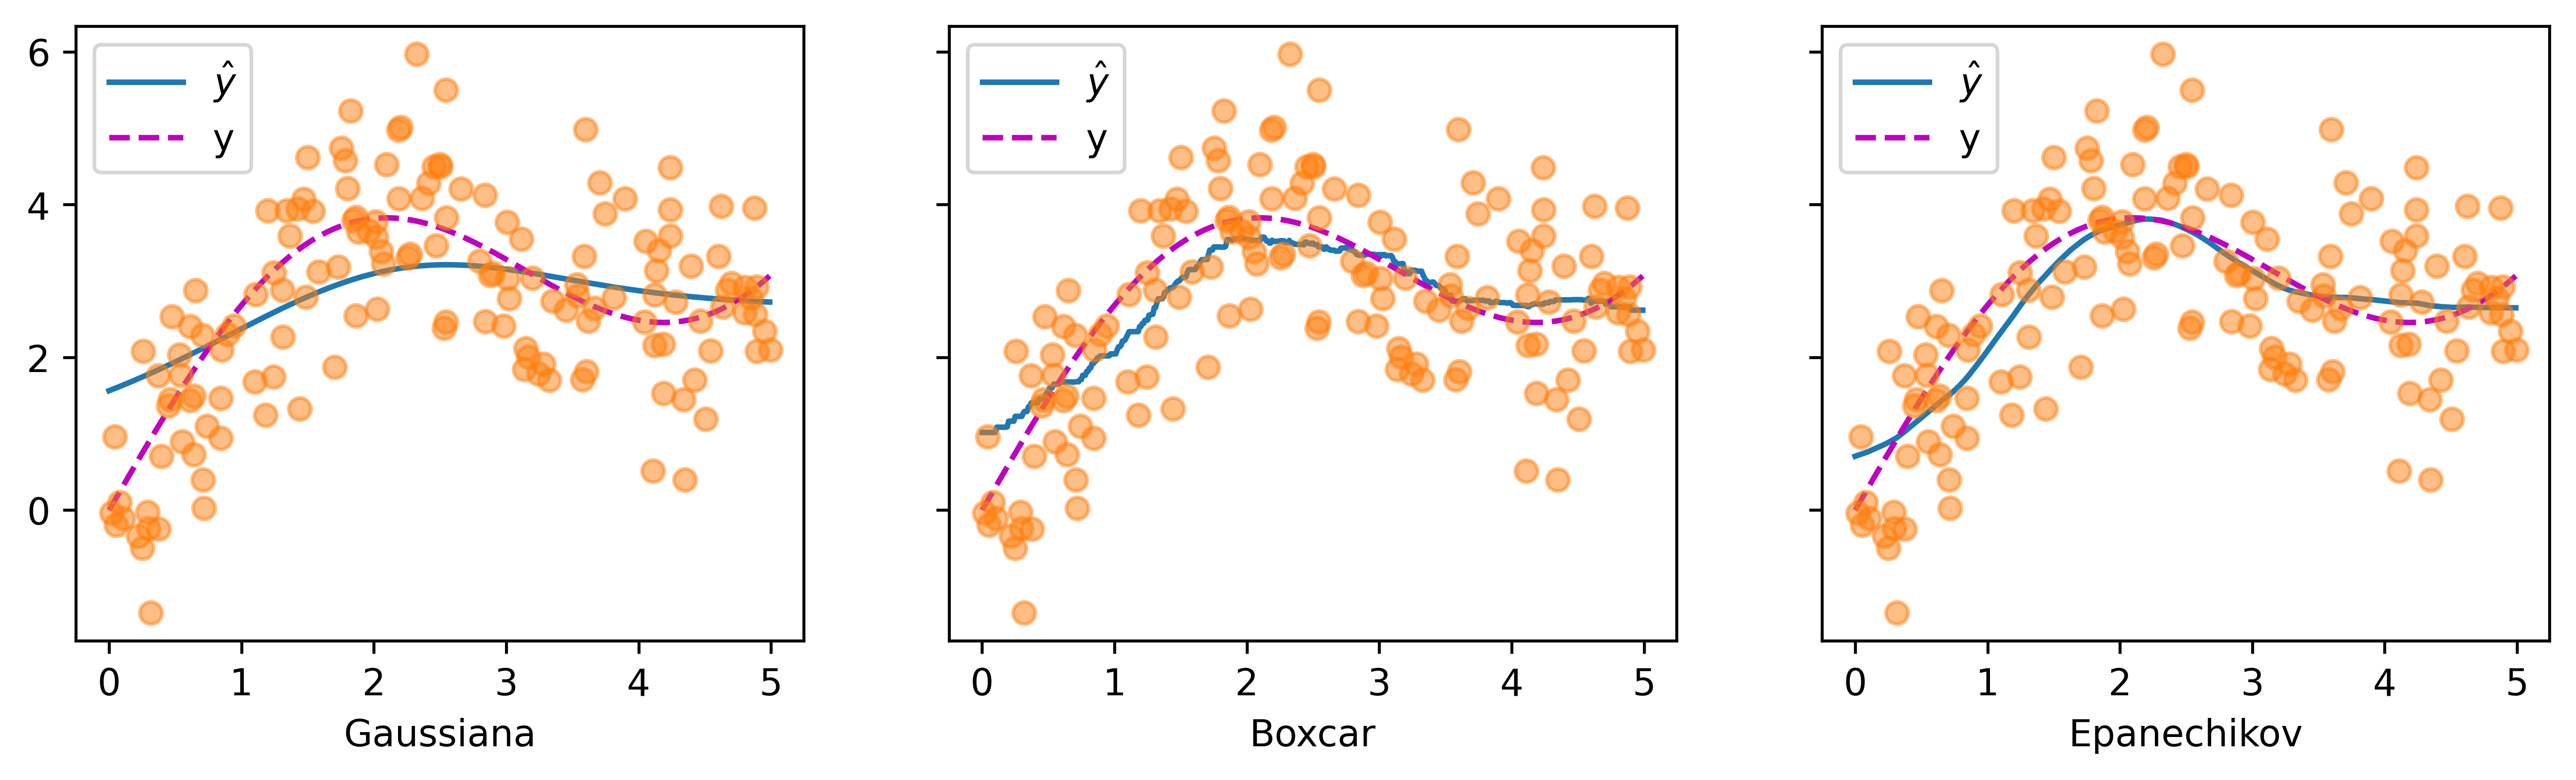
\includegraphics[width=\textwidth]{figures/chapter4/regression.png}
    \caption{Estimación de la función \( y \) mediante la estimación del valor de la variable objetivo sobre una partición equiespaciada del intervalo \( [0, 5] \) usando tres kérneles de similitud distintos.}
    \label{fig:regression}
\end{figure}

Esta forma de utilizar la atención es una forma de \textit{estimación de densidad de kernel}, una técnica clásica de inferencia no paramétrica que tiene la ventaja de que no requiere de ningún entrenamiento. Existen diversas heurísticas para elegir el \textit{kernel} \cite{silverman1986density} y puede probarse que si la anchura del \textit{kernel} se ajusta adecuadamente conforme se añaden observaciones entonces el método converge al valor real \( \E \llbracket y | x = x \rrbracket \) \cite{mack1982weak}.

\begin{figure}[tb]
    \centering
    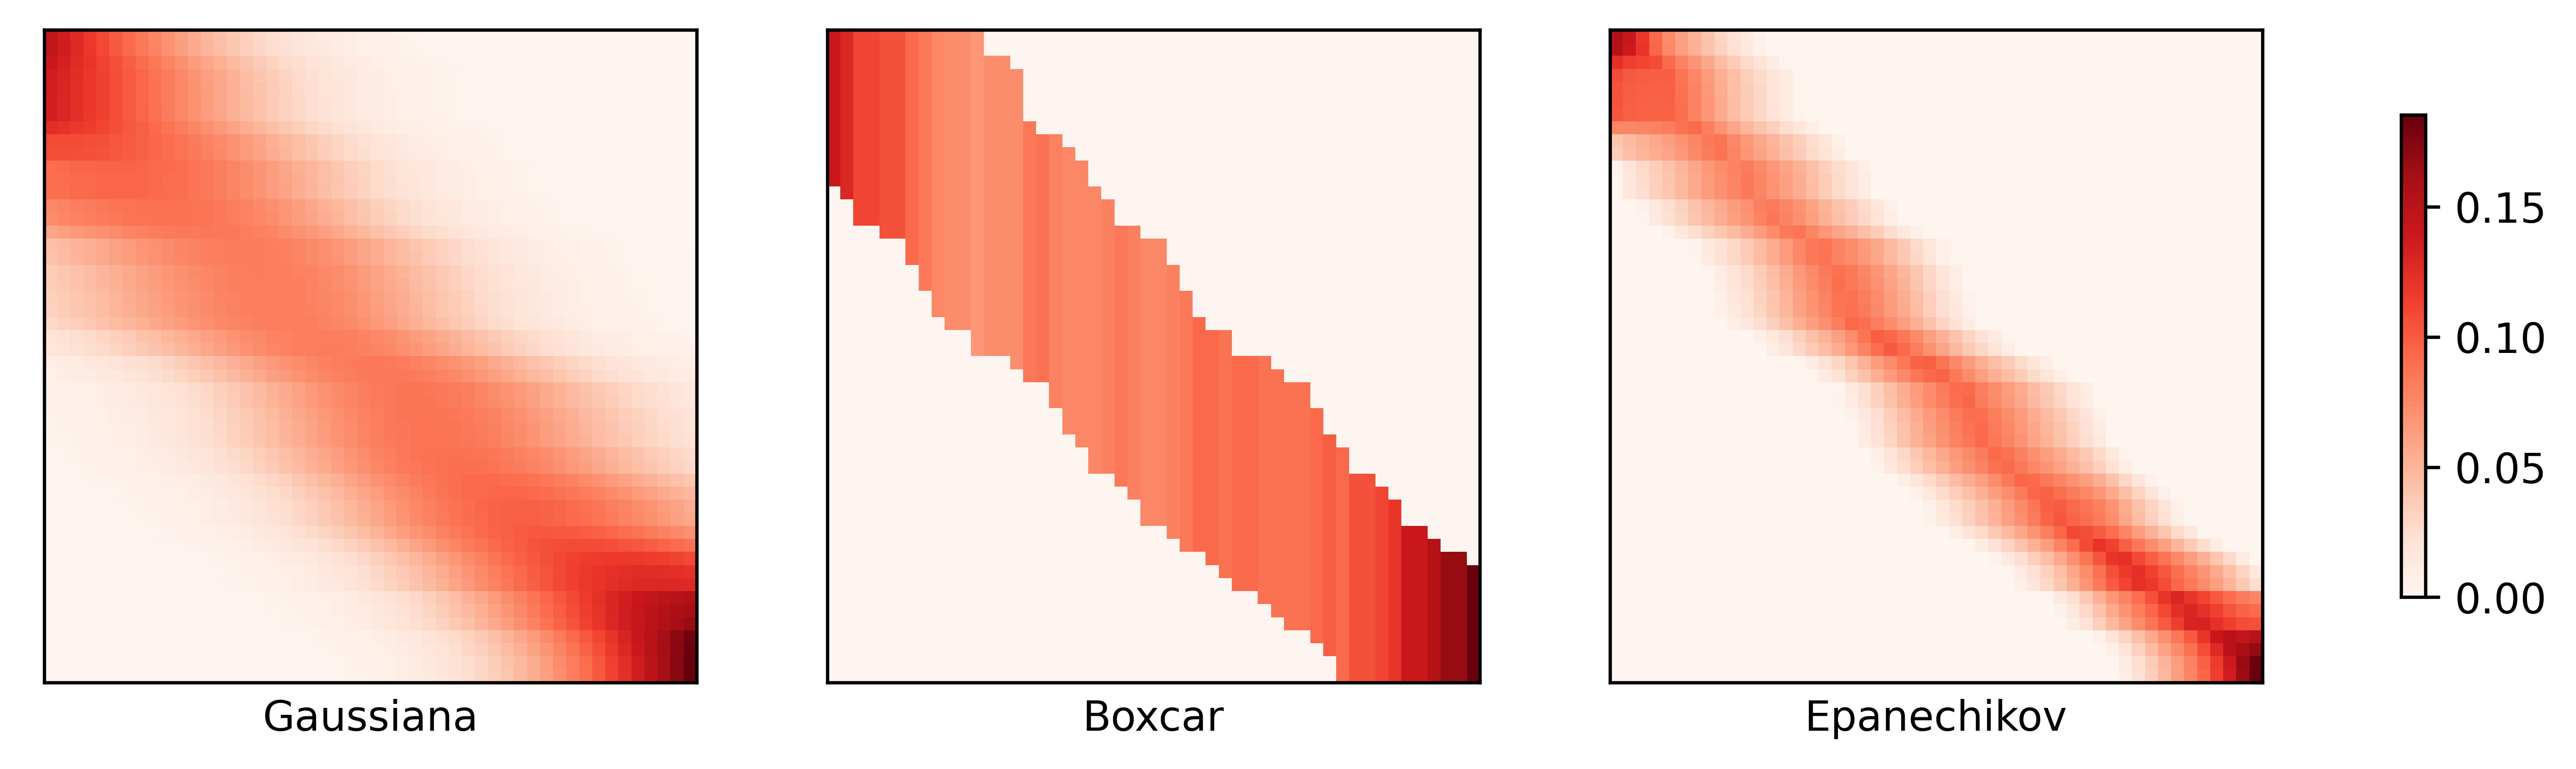
\includegraphics[width=\textwidth]{figures/chapter4/kernel.png}
    \caption{Visualización de los pesos de atención. Cada fila representa uno de los puntos aproximados y cada columna una componente del vector de atención. El color representa la magnitud de la componente.}
    \label{fig:kernel}
\end{figure}

El estudio del estimador de Nadaraya-Watson cumple un triple propósito: en primer lugar, muestra la flexibilidad de los métodos de atención y su relación con métodos clásicos de inferencia estadística. En segundo lugar, sirve para exhibir una de los grandes atributos de los métodos de atención: la posibilidad de visualizar los pesos de atención a fin de poder entender el funcionamiento del modelo. En tercer lugar, muestra lo decisivo de realizar una buena elección de la representación de la base de datos (claves y valores). En última instancia, la complejidad de elegir representaciones adecuadas lleva a diseñar esta representación de forma que sea \textit{aprendida} como una parte más de los parámetros del modelo.
